\section{PHƯƠNG TRÌNH MẶT CẦU}
\subsection{LÝ THUYẾT CẦN NHỚ}
\subsubsection{Định nghĩa}
\begin{itemize}
	\item [\iconCH] \immini{	Trong không gian, tập hợp tất cả các điểm $M$  cách điểm $I$ cố định một khoảng không đổi $r$ $(r>0)$  cho trước được gọi là mặt cầu tâm $I$ bán kính $R$. Kí hiệu $S(I;r)$ hay viết tắt là $(S)$. Vậy $S(I;R)=\{M|IM=r\}.$
		\item [\iconCH] Nhận xét: 
		\begin{itemize}
			\item Nếu $IM=r$ thì $M$ nằm trên mặt cầu.
			\item 	Nếu $IM<r$ thì $M$ nằm trong mặt cầu.
			\item 	Nếu $I M>r$ thì $M$ nằm ngoài mặt cầu.
		\end{itemize}
	}{\hspace{1cm}
		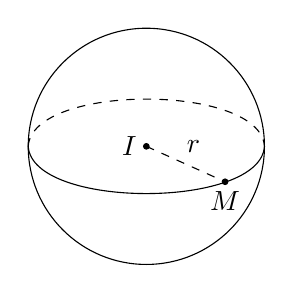
\begin{tikzpicture}
			\draw[fill=black] (0,0) circle(1pt) node[left]{$I$};
			\draw (0,0) circle(1.5);
			\draw (-1.5,0)..controls (-1.45,-0.8) and (1.45,-0.8)..(1.5,0);
			\draw[dashed] (-1.5,0)..controls (-1.45,0.8) and (1.45,0.8)..(1.5,0);
			\draw[dashed] (0,0)--(1,-0.45);
			\draw[fill=black] (1,-0.45) circle(1pt) node[below]{$M$};
			\node at (0.6,0) {$r$};
	\end{tikzpicture}}
\end{itemize}
\subsubsection{Phương trình mặt cầu}
\begin{itemize}
	\item [\iconCH] Trong khÔng gian $Oxyz$, mặt cầu $(S)$ tâm $I(a;b;c)$ bán kính $r$ có phương trình là $$(x-a)^2+(y-b)^2+(z-c)^2=r^2.$$
	\item [\iconCH] Dạng khai triển: $x^2+y^2+z^2-2ax-2by-2cz+d=0, \text{ với } d=a^2+b^2+c^2-r^2>0.$
\end{itemize}
\subsection{PHÂN LOẠI, PHƯƠNG PHÁP GIẢI TOÁN}
\begin{dang}{Xác định tâm $I$, bán kính $r$ của mặt cầu cho trước}
	\begin{itemize}
		\item [\iconCH] \indamm{Loại 1.} Cho $(S) \colon (x-a)^2+(y-b)^2+(z-c)^2=r^2$ . Khi đó
		\begin{listEX}[1]
			\item [\ding{172}] Tâm $I\left(a;b;c\right)$ (đổi dấu số trong dấu ngoặc);
			\item [\ding{173}] Bán kính $r$ (Rút căn vế phải).
		\end{listEX}
		\item [\iconCH] \indamm{Loại 2.} Cho $(S)\colon x^2+y^2+z^2-2ax-2by-2cz+d=0$. Khi đó
		\begin{listEX}[1]
			\item [\ding{172}] Điều kiện để (*) là mặt cầu là $a^2+b^2+c^2-d > 0$;
			\item [\ding{173}] Tâm $I\left(a,b,c\right)$ (đổi dấu hệ số của $x$, $y$, $z$ và chia đôi);
			\item [\ding{174}]  Bán kính $R=\sqrt{a^2+b^2+c^2-d}$ .
		\end{listEX}
	\end{itemize}
\end{dang}


\begin{dang}{Lập phương trình mặt cầu và ứng dụng thực tiễn}
	\begin{itemize}
		\item [\iconCH] \indamm{Phương pháp chung:} Cần xác định được tọa độ tâm $I\left(a;b;c\right)$ và độ dài bán kính $r$.
		\item [\iconCH] \indamm{Các bài toán cơ bản:}
		\begin{listEX}[1]
			\item [\ding{172}] Mặt cầu có tâm $I\left(a;b;c\right)$ và đi qua điểm $A\left(x_A;{y_A};{z_A}\right)$ thì bán kính $$r=IA=\sqrt{\left(x_A-x_I\right)^2+\left(y_A-y_I\right)^2+\left(z_A-z_I\right)^2}.$$
			\item [\ding{173}] Mặt cầu (S) có đường kính $AB$ thì
			\begin{itemize}
				\item [$\bullet$] Tâm $I\left(a;b;c\right)$ là trung điểm của $AB$ hay $I\left(\dfrac{x_A+x_B}{2};\dfrac{y_A+y_B}{2};\dfrac{z_A+z_B}{2}\right)$.
				\item [$\bullet$] Bán kính $r=\dfrac{AB}{2}=\dfrac{\sqrt{\left(x_B-x_A\right)^2+\left(y_B-y_A\right)^2+\left(z_B-z_A\right)^2}}{2}$.
			\end{itemize}
			\item [\ding{174}] Mặt cầu có tâm $I(a;b;c)$ và tiếp xúc với $(\alpha) \colon Ax+By+Cz+D=0$ thì bán kính $$r=\mathrm{d}\left(I,(\alpha) \right)= \dfrac{\big|Aa+Bb+Cc+D\big|}{\sqrt{A^2+B^2+C^2}}.$$
			\item [\ding{175}] Mặt cầu qua bốn điểm $A$, $B$, $C$, $D$ không đồng phẳng (ngoại tiếp tứ diện $ABCD$)\\
			Gọi $(S)$ có dạng $x^2+y^2+z^2-2ax-2by-2cz+d=0$ (*)\\
			Thay tọa độ 4 điểm $A$, $B$, $C$, $D$ vào (*), ta được hệ phương trình 4 ẩn số $a$, $b$, $c$, $d$;\\
			Giải tìm $a$, $b$, $c$, $d$. Suy ra tâm $I\left(a,b,c\right)$ , bán kính $R=\sqrt{a^2+b^2+c^2-d}$.
		\end{listEX}
	\end{itemize}
\end{dang}


\begin{dang}{Vị trí tương đối của điểm, của mặt phẳng với mặt cầu}
	\begin{enumerate}[\iconCH]
		\item \indamm{Bài toán 1:} Xét điểm $M(x_0;y_0;z_0)$ và mặt cầu $S \colon (x-a)^2+(y-b)^2+(z-c)^2-r^2=0 \quad (1)$. Thay tọa độ điểm $M$ vào vế trái của (1), nếu
		\begin{listEX}[1]
			\item [\ding{172}] Kết quả bằng $0$ thì $M \in (S)$.
			\item [\ding{173}] Kết quả ra số âm thì $M$ nằm trong $(S)$.
			\item [\ding{174}] Kết quả ra số dương thì $M$ nằm trong $(S)$.
		\end{listEX}
		\item \indamm{Bài toán 2:} Cho mặt cầu $(S)$ có tâm $I(a;b;c)$, bán kính $r$ và mặt phẳng $(P)\colon Ax+By+Cz+D=0$.
		\begin{tcolorbox}[colframe=orange!3,colback=red!3!white,boxrule=0.2mm]
			\begin{listEX}[1]
				\item [\ding{172}] Nếu $\mathrm{d}\left(I,(P) \right)=\dfrac{\bigg|Aa+Bb+Cc+D\bigg|}{\sqrt{A^2+B^2+C^2}}>r$ thì $(P)$ và $(S)$ không có điểm chung.
				\item [\ding{173}] Nếu $\mathrm{d}\left(I,(P) \right)=\dfrac{\bigg|Aa+Bb+Cc+D\bigg|}{\sqrt{A^2+B^2+C^2}}=r$ thì $(P)$ tiếp xúc $(S)$.
				\item [\ding{174}] Nếu $\mathrm{d}\left(I,(P) \right)=\dfrac{\bigg|Aa+Bb+Cc+D\bigg|}{\sqrt{A^2+B^2+C^2}}<r$ thì $(P)$ cắt $(S)$.
			\end{listEX}
		\end{tcolorbox}
	\end{enumerate}
\end{dang}


